\documentclass[11pt,twoside]{article}
\usepackage[margin=1in]{geometry}
\usepackage[T1]{fontenc}
\usepackage[nott,notextcomp]{kpfonts}
\usepackage{fancyhdr}
\usepackage{lastpage}
\usepackage{hyperref}
\usepackage{listings}
\usepackage{enumitem}
\usepackage{scrextend}

\usepackage{graphicx,epstopdf}
\epstopdfsetup{update}
\DeclareGraphicsExtensions{.ps}
\epstopdfDeclareGraphicsRule{.ps}{pdf}{.pdf}{ps2pdf -dEPSCrop -dNOSAFER #1 \OutputFile}

\newcommand{\inlinecode}{\texttt}

% Some breathing room between paragraphs
% \setlength{\parskip}{.5\baselineskip}%

% Page layout: stretch text to fill up page.
\addtolength\footskip{.25\headheight}
\flushbottom

% Headings.
\pagestyle{fancy}
\let\headrule\empty
\let\footrule\empty
\lhead{\scshape CSC\,469}
\chead{\large\scshape Assignment \#\,2}
\rhead{\scshape Fall 2016}
\cfoot{\scshape page \thepage\space of \pageref{LastPage}}

\begin{document}
\title{CSC469 A2: Concurrency}
\author{\textsc{Cheung}, Eugene Yue-Hin (cheun550) and \textsc{Snyder}, Eric (snyderer)}
\date{2016-11-13}
\maketitle


\section{Introduction}
In order to design a parallel memory allocator, we must place importance on good speed, good scalability, no false sharing, and low fragmentation. Since these goals were outlined and achieved by the Hoard memory allocator by Berger et al. \cite{hoard}, it was chosen as the base design for our program. The Hoard memory allocator achieves this by having separate private heaps for each CPU thread and a global heap that can be used to distribute allocatable space. Each heap uses page-aligned superblocks which encapsulates smaller blocks of a fixed size. If a heap runs out of free blocks, a new superblock can be obtained from the global heap, or, if the global heap is empty the \inlinecode{sbrk()} function can be used to allocate more space to create a new superblock. Any time a CPU heap crosses beyond a certain emptiness threshold, a suitably empty superblock is returned to the global heap, which can then be handed out to another heap when needed. Large memory requests are handled by the OS to avoid overhead.


\section{Design}
We were given a short list of requirements that our allocator must adhere to: it all had to fit inside a single file (not an issue), we could not statically allocate large data structures for the heap (Hoard doesn't do this) and we could assume that each thread making requests of our allocator would execute exclusively on a single CPU (compared to Hoard, we only have one heap per CPU). While it is clear that there are better options than Hoard \cite{jemalloc}, Hoard's design is a relatively good balance of a simple design and performance. Likewise, the alternative free list design \cite{notes} seems simpler, but the lack of bins and fullness sizes as outlined in Hoard suggested that it may not perform as well.

Our design uses heaps, one for each CPU as stated above, which store a linked list of pointers to different bins of superblocks. There is a bin of superblocks for each fullness size class to make finding an appropriate superblock faster. Each superblock contains metadata, including pointers to the next/previous superblock within its linked list. The size of our superblocks are 4096 bytes, which is the typical size of a system page. These blocks are then divided into sizes from 8 to 2048 bytes, going up by logarithmically.

The heap struct contains the following:

\begin{itemize}
    \item
    \inlinecode{pthread\_mutex\_t lock}: A lock to prevent multiple threads from accessing the same heap at the same time.
    
    \item
    \inlinecode{int allocated}: Total number of bytes allocated in this heap (i.e. number of superblocks $\times$ page size.

    \item
    \inlinecode{int used}: Total number of bytes used in the heap's superblocks.
    
    \item
    \inlinecode{superblock\_t *bins[NSIZES][NBINS]}: 2D array of superblock pointers, where there are $NBINS$ number of fullness bins for all $NSIZES$ number of size classes.
\end{itemize}


The superblock struct contains the following:

\begin{itemize}
    \item
    \inlinecode{pthread\_mutex\_t lock}: A lock to prevent multiple threads from accessing the same superblock at the same time.

    \item
    \inlinecode{int owner}: ID of the superblock's owner heap.
    
    \item
    \inlinecode{int size\_class\_idx}: The index of the corresponding size class in the static \inlinecode{SIZES} array.
    
    \item
    \inlinecode{int used}: Bytes used in the superblock.
    
    \item
    \inlinecode{int bitmap}: A bitmap used to track which blocks are currently in use.
    
    \item
    \inlinecode{struct superblock *prev/struct superblock *next}: Pointers to the previous and next superblocks in the bin.
\end{itemize}

\subsection{mm\_malloc}
If the size requested is deemed "large" (i.e. larger than any of the specified size classes), we simply use the system \inlinecode{malloc()} function to handle it. However, if we need to handle the allocation, then we follow the design as described by Berger et Al. As aforementioned, our design is simplified to assume each thread is associated with only a single unique CPU, so our \inlinecode{hash()} function simply determines which CPU was used to call \inlinecode{mm\_malloc()} in order to figure out which heap to use. The allocator then looks for a sufficiently free superblock in the heap based on the size class. If none is found, it then scans the global heap's bins to transfer one to the current heap. If still none is found, a new superblock is allocated. Note that the superblock metadata is placed at the beginning of the superblock, which leads to some internal fragmentation. Next, we find a free block within the superblock and mark it as used in the bitmap. We transfer the superblock to the appropriate fullness bin and return a pointer to the chosen block.

\subsection{mm\_free}
Our free function works by first checking to see if the pointer is to memory that we allocated or that the system handled (for large allocations). By performing a modulo operation on the pointer and the page size we can move up to the closest page border to read the superblock header. Now that we have the superblock we can also lock the heap that owns it so we can begin the free operation. We use \inlinecode{memset} to simply zero the block in memory and mark it as free in the bitmap. The superblock is then moved to the appropriate fullness bin, if needed. We then check to see if the heap is "too empty" and if so transfer a mostly empty superblock from the heap to the global heap. At this point, we are done with freeing and can unlock everything.


\section{Analysis}
Four benchmarks were run on the allocators in order to test their active/passive false runtimes, and efficiency/throughput. These benchmarks were provided to us and were not modified in any way. The data described in this section are comparisons of the data from running our a2alloc allocator on the testing server and the data for libc and kheap provided on CDF. Note that the provided data set seemed to have the kheap numbers duplicated as the libc numbers, so all the graphs only contain two lines. The line that is \textit{not} a2alloc is in fact for kheap. 

\subsection{Cache Scratch}
\begin{figure}[!htbp]
    \centering
    \includegraphics[width=0.8\textwidth]{cache-scratch.ps}
    \caption{Results of cache-scratch.}
    \label{fig:scratch}
\end{figure}

We can see the results of the cache-scratch benchmark in Figure \ref{fig:scratch}. Both kheap and our a2alloc implementation perform similarly with a single thread, but then deviates after that. While kheap shows a sharp increase in runtime with 2 threads, then gradually decreases, our allocator shows a ~1 second decrease in runtime with 2 threads, then a gradual decline thereafter. libc should perform better (although not as significant of a difference as that of between kheap and a2alloc) than our allocator. We can see that with a higher number of threads, our a2alloc implementation is around 1.5 seconds faster than kheap.

\subsection{Cache Thrash}
\begin{figure}[!htbp]
    \centering
    \includegraphics[width=0.8\textwidth]{cache-thrash.ps}
    \caption{Results of cache-thrash.}
    \label{fig:thrash}
\end{figure}

The results of the cache thrash benchmark, which can be seen in Figure \ref{fig:thrash} are similar to those of the previous cache scratch benchmark. Single-threaded performance performs close (although slightly better) and double-threaded performance for ours marking a sharp improvement in the runtime whereas the runtime of kheap becomes much worse. Both allocators for 3+ number of threads slowly begin to decrease. libc appears to be similar in terms of trends to our a2alloc but with the runtime generally being slightly better, generally forming a similar looking line twice with the libc being slightly below ours. Similar to the cache scratch benchmark, we can see that with a higher number of threads, our a2alloc implementation is around 1.5 seconds faster than kheap.

\subsection{Larson}
\begin{figure}[!htbp]
    \centering
    \includegraphics[width=0.8\textwidth]{larson.ps}
    \caption{Results of larson.}
    \label{fig:larson}
\end{figure}

This test induces heavy fragmentation by repeatedly spawning threads to allocate and free blocks in random orders. Compared to libc, which increases in performance generally linearly with the number of threads, our performance is somewhat "S" shaped, with single threaded performance being great but the 2-4 core range seemingly dropping to kheap levels before returning to a somewhat linear increase (though not quite as efficient as libc), as seen in Figure \ref{fig:larson}.

\subsection{Threadtest}
\begin{figure}[!htbp]
    \centering
    \includegraphics[width=0.8\textwidth]{threadtest.ps}
    \caption{Results of threadtest.}
    \label{fig:threadtest}
\end{figure}

Finally, the results of the threadtest benchmark can be seen in Figure \ref{fig:threadtest}. This test runs $t$ threads repeatedly and allocates/deallocates $K/t$ blocks of given size. Our performance on this test is actually worse than kheap on 1 thread but where kheap starts to grow dramatically, we drop before increasing again a bit. libc starts below either of these and trends downwards slowly. Combined with our results in larson we suspect that there might be an issue with our multithreading implementation causing some poor performance on certain numbers of thread, potentially related to locking.


\section{Discussion}
While we are generally happy with how our allocator performs when compared to kheap, there are definitely rooms for improvement when compared to libc. Short of a drastic redesign to more closely mimic decisions made by other implementations such as jemalloc, there a few improvements that could have been made to ours if time was not a limiting factor (listed in no particular order):

\begin{enumerate}
    \item
    Lower fragmentation could be achieved by better handling superblock metadata. Since the metadata sits at the beginning of the superblock, we mark the blocks that it takes up as used. However, if the size class is larger than the size of the superblock size, then the block used by the superblock will contain empty space. For example, a superblock of size class 2048 bytes will have two blocks, but the first one will be used solely for the metadata, leaving a large amount of empty space between the superblock metadata and the sole "usable" data block. The allocator could be modified to make use of the empty space, although that would complicate the logic behind the size classes.
    
    \item
    More compact structs would allow for lower memory usage. While we are using \inlinecode{int}s for various values in our superblock and heap structs, it is possible to choose smaller data types if we assume page size and consequent upper bounds of the values. For example, the superblock bitmap would only need to be a maximum of 512 bits if the smallest size class is 8 bytes and a page is 4096 bytes. These optimizations were not done in the interest of time and having a simpler program for reading/debugging purposes.
    
    \item
    Lower memory usage could likely be achieved with more fine-tuned thresholds per size class. While we chose a value of 8 for the $K$ value (as defined in the Hoard algorithm), it was done so somewhat arbitrarily by eyeballing results of running the provided benchmarks on a lightly loaded CDF/CSSU server (\inlinecode{theo.teach.cs.toronto.edu}; 24 $\times$ Intel(R) Xeon(R) CPU X5690 @ 3.47GHz, 96 GB RAM).
    
    \item
    A design that relies less on locks would be more efficient due to less contention. Per-thread caching mechanisms would allow for less locking, and thus less overhead.
    
    \item
    Since we assume that a page is 4096 bytes, the size classes were chosen to be powers of 2 between 8 and 2048. To have better portability, the size classes would need to be dynamically generated based on the page size returned by \inlinecode{mem\_pagesize()}. On a related note, jemalloc uses more size classes than we chose, which could also lead to less fragmentation due to better usage of memory blocks (also mentioned in the article about dlmalloc \cite{dlmalloc}). dlmalloc also has more bins for sizes smaller than 512 bytes because they "tend to produce the least fragmentation on real loads," although our benchmarking tests are arguably unlike real loads.
\end{enumerate}


\begin{thebibliography}{4}

% https://people.cs.umass.edu/~emery/pubs/berger-asplos2000.pdf
\bibitem{hoard} 
Berger, E. D., Mckinley, K. S., Blumofe, R. D., & Wilson, P. R. (2000). Hoard. \textit{ACM SIGARCH Computer Architecture News SIGARCH Comput. Archit. News, 28}(5), 117-128. doi:10.1145/378995.379232

% https://www.facebook.com/notes/facebook-engineering/scalable-memory-allocation-using-jemalloc/480222803919
\bibitem{jemalloc}
Evans, J. (2011, January 3). Scalable memory allocation using jemalloc. Retrieved November 12, 2016, from https://www.facebook.com/notes/facebook-engineering/scalable-memory-\\allocation-using-jemalloc/480222803919

% http://g.oswego.edu/dl/html/malloc.html
\bibitem{dlmalloc}
Lea, D. (n.d.). A Memory Allocator. Retrieved November 12, 2016, from http://g.oswego.edu/dl/html/malloc.html

% http://www.teach.cs.toronto.edu/~csc469h/fall/assignments/a2/malloc_notes.pdf
\bibitem{notes}
Simion, B. (n.d.). Malloc notes. Retrieved November 12, 2016, from http://www.teach.cs.toronto.edu/~csc469h/fall/assignments/a2/malloc\_notes.pdf

\end{thebibliography}

\end{document}
